%class
	\documentclass{beamer}

%template
	\usetheme{HannoverSalman}
	\setbeamertemplate{navigation symbols}{}
	%\setbeamertemplate{footline}{\centering{\insertframenumber/\insertpresentationendpage}}
	%\setbeamertemplate{footline}{\hspace*{.5cm}\scriptsize{\hfill\insertframenumber\hspace*{.5cm}}} 


%packages
	\usepackage{amsmath, amssymb, graphicx,cancel}
	\usepackage[absolute,overlay]{textpos}
	\usepackage{subfigure}
	\usepackage{caption}\captionsetup{labelformat=empty,labelsep=none}
	\usepackage{geometry}
	\geometry{verbose}
	\usepackage{color}
	\usepackage{xmpmulti}
	\usepackage[3D]{movie15}
	\usepackage{hyperref}
%	\usepackage{bookmark}
	\usepackage[open,openlevel=4,atend]{bookmark}
	%\bookmarksetup{color=blue}
	\usepackage{multirow}
	\usepackage[style=numeric,defernumbers, authoryear]{biblatex}
	%\usepackage[square,sort]{natbib}
	%\usepackage{fancyhdr}%\pagestyle{fancy} 

	
	\hypersetup{bookmarksdepth = 4}


%citations files
	\bibliography{MyCitations}

%logoCSIPCPL
    \setlength{\TPHorizModule}{1mm}
    \setlength{\TPVertModule}{1mm}
    \newcommand{\logoCSIPCPL}
    {
    	\begin{textblock}{1}(100,2) %(100,85)  for bottom
    		
\includegraphics[width=1.5cm]{figs/logo_CSIP}
    	\end{textblock}
    	
	\begin{textblock}{1}(117,1) %(117,85)  for bottom
    		
\includegraphics[width=1.0cm]{figs/logo_CPL}
    	\end{textblock} 
    }

%logo evolution
    \newcommand{\logoEvolution}
    {    	
	\begin{textblock}{1}(110,1) %(117,85)  for bottom
    		\includegraphics[width=0.65in]{figs/logo_evolution.pdf}
    	\end{textblock} 
    }

%logo Qualcomm
    \newcommand{\logoQualcomm}
    {
    	\begin{textblock}{1}(110,2) %(100,85)  for bottom
    		\includegraphics[width=1.5cm]{figs/logo_qualcomm.jpg}
    	\end{textblock}
    }
%logo Qualcomm (long)
    \newcommand{\logoQualcommllong}
    {
    	\begin{textblock}{1}(0,0) 
    		\includegraphics[width=1.25in]{figs/logo_qualcomm_long.jpg}
    	\end{textblock}
    }

%logo Tech Tower
    \newcommand{\logoTechTower}
    {
    	\begin{textblock}{1}(0,0) 
    		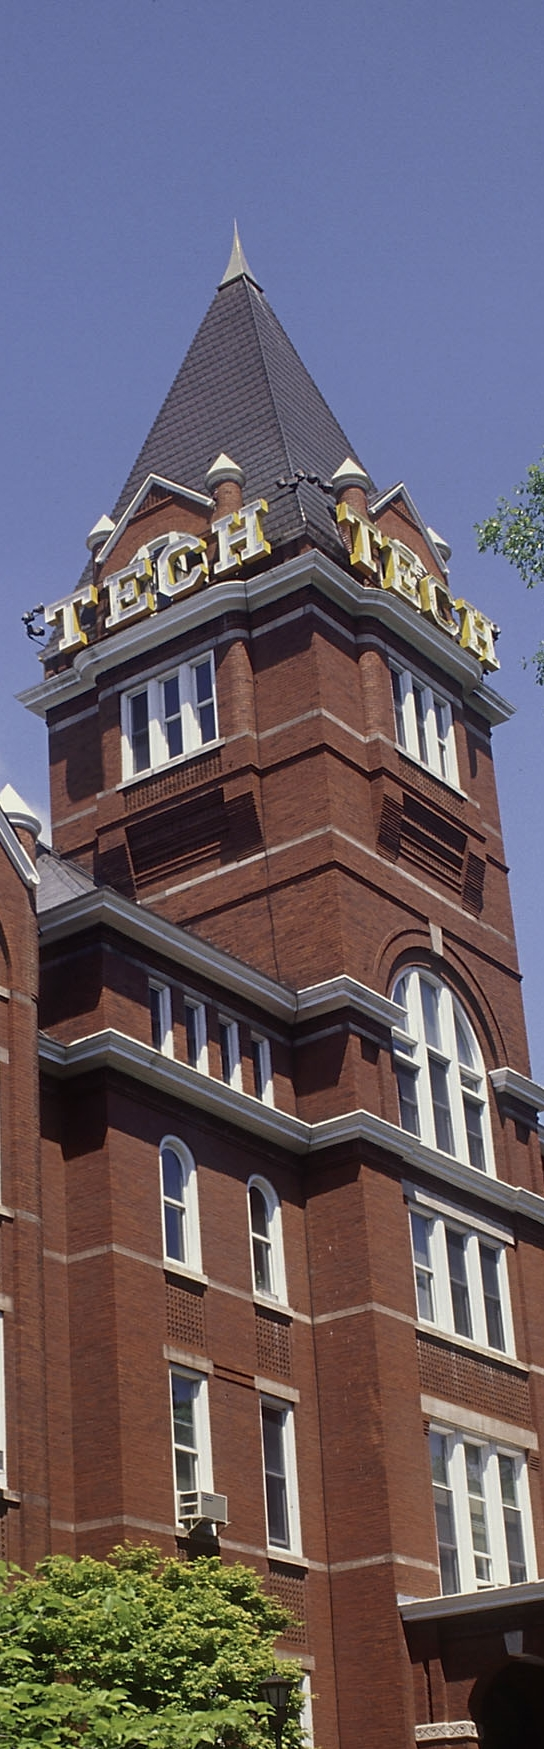
\includegraphics[width=1.25in]{figs/logo_TechTower.jpg}
    	\end{textblock}
    }

%logo tree
    \newcommand{\logoTree}
    {
    	\begin{textblock}{1}(0,0) 
    		\includegraphics[width=1.25in]{figs/logo_tree.jpg}
    	\end{textblock}
    }
%page numbers
    \newcommand{\mypagenum}
    {
    	\begin{textblock}{1}(1,94) 
		{\tiny \color[rgb]{0.2,0.2,1}\insertframenumber} %\insertframenumber,\insertpresentationendpage, \inserttotalframenumber
    	\end{textblock}
    }
%my footnote citation
	\newcommand{\myFootnoteCitation}[2]
	{
		\footnote{\tiny \citeauthor{#1}, \emph{#2}, \citeyear{#1}.}  %\citeauthor{#1}, \citetitle{#1}, #2 \citeyear{#1}.
	}
%my refer to citation
	\newcommand{\mycite}[1]
	{
		\emph{\citeauthor{#1} (\citeyear{#1})}
	}
%my footnote website citation
	\newcommand{\myFootnoteWebsiteCitation}[1]
	{
		\footnote{\tiny \citeauthor{#1}}
	}

\let\thefootnote\relax\footnotetext{Footnotetext without footnote mark}


%section underline
%\newcommand{\tmpsection}[1]{}
%\let\tmpsection=\section
%\renewcommand{\section}[1]{\tmpsection{\underline{#1}}}



%commands
	\newcommand{\likelihood}{p(Z_k| x_k) }						%likelihood
	\newcommand{\prior}{p(x_k)  } 								%prior
	\newcommand{\posterior} {p(x_k| Z_k)}						%posterior
	\newcommand{\prediction} {p(x_k| Z_{k-1})}					%prediction
	\newcommand{\update} {p(x_k|Z_k)}							%update
	\newcommand{\observations} {p(Z_k)}						%observations
	\newcommand{\prevobservations} {p(Z_{k-1})}				%previous observations
	\newcommand{\dxpk} {dx_{k-1}}							%dx_{k-1}
	\newcommand{\ChapKolm}{\int{p(x_k| x_{k-1})p(x_{k-1}|Z_{k-1})} \dxpk} %Chapman Kolmogorov

	%algorithm specific: JPDAF
	\newcommand{\likelihoodJPDAF}{p(Z_k| \chi, m, Z_{k-1}) }		%1. likelihood
	\newcommand{\priorJPDAF}{p(\chi|m, Z^{k-1}} 				%2. prior	
	\newcommand{\observationsJPDAF} {p(Z_k}					%3. observations
	\newcommand{\posteriorJPDAF} {p(\chi| Z_k)}					%4. posterior

%environments
	\newenvironment{changemargin}[2]
	{
	  	\begin{list}{}
		{
			\setlength{\topsep}{0pt}%
			\setlength{\leftmargin}{#1}%
			\setlength{\rightmargin}{#2}%
			\setlength{\listparindent}{\parindent}%
			\setlength{\itemindent}{\parindent}%
			\setlength{\parsep}{\parskip}%
		}
	  	\item[]
		}
		{\end{list}
	}
%figures

%colors
\definecolor{darkgreen}{rgb}{0,0.5,0}

%personal details
	\author{Salman Aslam}
	\institute{Advisor, Dr Christopher Barnes (ECE)\\Co-advisor, Dr Aaron Bobick (CoC)\\Georgia Institute of Technology}
	\date{}

\begin{document}
%####################################################################################################
\title{Human tracking}
%####################################################################################################
\begin{frame}[plain]\logoTechTower
	\titlepage
\end{frame}

\begin{frame}
\frametitle{Outline}
\logoCSIPCPL\logoTechTower
	\setcounter{tocdepth}{1}	
	\tableofcontents
\end{frame}

%#######################################################################
\section{INTRODUCTION}
%#######################################################################
\begin{frame}
\frametitle{Introduction}
\framesubtitle{}
\logoCSIPCPL\mypagenum
\end{frame}


%#######################################################################
\section{PRIOR WORK}
%#######################################################################
\begin{frame}
\frametitle{Prior work}
\framesubtitle{}
\logoCSIPCPL\mypagenum
\end{frame}


%=================================
\subsection{2000: W4 (Haritaoglu)}
%=================================
\begin{frame}
\frametitle{Prior work: W4}
\framesubtitle{1. overview}
\logoCSIPCPL\mypagenum
\myFootnoteCitation{2000_JNL_W4_Haritaoglu}{PAMI}
	%\begin{figure}
	%	\includegraphics[width=1.0\textwidth]{tables/TrackingPapers_SubspaceTracking_2006_PCA_Hog.pdf}
	%\end{figure}
\end{frame}



\begin{frame}
\frametitle{Prior work: W4}
\framesubtitle{2. summary}
\logoCSIPCPL\mypagenum
\myFootnoteCitation{2000_JNL_W4_Haritaoglu}{PAMI}
	\begin{itemize}
		\item static shape model
	\end{itemize}
\end{frame}




\begin{frame}
\frametitle{Prior work: W4}
\framesubtitle{figures}
\mypagenum
\myFootnoteCitation{2000_JNL_W4_Haritaoglu}{PAMI}
	\begin{figure}
		\includegraphics[width=1.0\textwidth]{figs/TrackingPapers_pedestrianTracking_2000_Haritaoglu_fig1.jpg}
	\end{figure}
\end{frame}
%============================
\subsection{2001: BRAmblE (Isard)}
%============================
\begin{frame}
\frametitle{Prior work: BRAmblE (Isard)}
\framesubtitle{2. summary}
\mypagenum
	\begin{itemize}
		\item unified approach to background/foreground modeling
	\end{itemize}
\myFootnoteCitation{2001_CNF_TRKhuman_Isard}{ICCV}
\end{frame}



%=================================
\subsection{2002: color particle filter (Perez)}
%=================================
\begin{frame}
\frametitle{Prior work: particle filter}
\framesubtitle{2. summary}
\mypagenum
	\begin{itemize}
		\item color histogram distance but within a probabilistic framework
		\item populate an HS histogram only with pixels with S and V values larger than 0.1 and 0.2 respectively
		\item remaining "color-free" pixels populate value only bins, crucial for tracking black and white regions
		\item multi-part color modeling to capture rough spatial layout ignored by global histograms
		\item incorporation of a background color model when appropriate
	\end{itemize}
\myFootnoteCitation{2002_CNF_TRKcolor_Perez}{ECCV}
\end{frame}



\begin{frame}
\frametitle{Prior work: particle filter}
\framesubtitle{2. summary (cont.)}
\mypagenum
	\begin{itemize}
		\item no restriction on class of shapes
		\item Bhattacharyya similarity coefficient, contrary to KL divergence,
			\begin{itemize}
				\item "proper"
				\item within $[0,1]$
				\item empty bins not a problem
			\end{itemize}
		\item when tracking multiple targets, two possible relative depth orderings of the two objects are assumed equally likely
		\item splitting ROI into {\color{blue}2} parts with individual color models
	\end{itemize}
\myFootnoteCitation{2002_CNF_TRKcolor_Perez}{ECCV}
\end{frame}
%=================================
\subsection{2004: crowded (Zhao)}
%=================================
\begin{frame}
\frametitle{Prior work: crowded (Zhao)}
\framesubtitle{1. overview}
\logoCSIPCPL\mypagenum
\myFootnoteCitation{2004_JNL_TRK_shape_Zhao}{PAMI}
	%\begin{figure}
	%	\includegraphics[width=1.0\textwidth]{tables/TrackingPapers_SubspaceTracking_2006_PCA_Hog.pdf}
	%\end{figure}
\end{frame}




\begin{frame}
\frametitle{Prior work: crowded (Zhao)}
\framesubtitle{2. summary}
\logoCSIPCPL\mypagenum
\myFootnoteCitation{2004_JNL_TRK_shape_Zhao}{PAMI}
	\begin{itemize}
		\item prior locomotion model to assist posture estimation
	\end{itemize}
\end{frame}



\begin{frame}
\frametitle{Prior work: crowded (Zhao)}
\framesubtitle{3. comparison}
\logoCSIPCPL\mypagenum	
\myFootnoteCitation{2004_JNL_TRK_shape_Zhao}{PAMI}	
	\begin{itemize}
		\item difficulties with blob-based analysis (see pg \pageref{fig:1})
			\begin{enumerate}
				\item a single blob may contain multiple humans due to their physical proximity or due to camera viewing angle
				\item a single object may be fragmented into several blobs due to low color contrast 
				\item blobs may contain pixels corresponding to shadows or reflections
			\end{enumerate}
				\item blobs may go through frequent structural changes (split and merge) due to above problems
				\item this causes combinatorial search for temporal correspondence
				\item even if correspondence is established, what each trajectory corresponds to (e.g. object, part of an object, a few objects together) is still unknown
	\end{itemize}
\end{frame}




\begin{frame}
\frametitle{Prior work: crowded (Zhao)}
\framesubtitle{3. comparison (cont.)}
\logoCSIPCPL\mypagenum	
\myFootnoteCitation{2004_JNL_TRK_shape_Zhao}{PAMI}
	\begin{itemize}
		\item advantages of shape based approach used
			\begin{enumerate}
				\item detecting individual objects is a goal
				\item real entities do not undergo structural changes such as split and merge
				\item constraints on (e.g. shape, size, motion) can assist segmentation and tracking
				\item less sensitive to noise and parameters of low-level processing
				\item a camera model provides additional constraints
			\end{enumerate}
	\end{itemize}
\end{frame}


\begin{frame}
\frametitle{Prior work: crowded (Zhao)}
\framesubtitle{4. contributions}
\logoCSIPCPL\mypagenum
\myFootnoteCitation{2004_JNL_TRK_shape_Zhao}{PAMI}
\end{frame}


\begin{frame}
\frametitle{Prior work: crowded (Zhao)}
\framesubtitle{5. methodology: overview}
\logoCSIPCPL\mypagenum
\myFootnoteCitation{2004_JNL_TRK_shape_Zhao}{PAMI}
	\begin{enumerate}
		\item change detection
		\item human hypotheses are computed by boundary and shape analysis using human shape and camera model
		\item each hypothesis is tracked in 3D in the subsequent frames with a Kalman filter using the object's appearance constrained by its shape
		\item 2D positions are mapped onto the 3D ground plane and trajectories are formed and filtered in 3D
	\end{enumerate}
\end{frame}



\begin{frame}
\frametitle{Prior work: crowded (Zhao)}
\framesubtitle{5. methodology: detailed}
\logoCSIPCPL\mypagenum
\myFootnoteCitation{2004_JNL_TRK_shape_Zhao}{PAMI}
	\begin{enumerate}\setcounter{enumi}{0}
		\item change detection
			\begin{itemize}
				\item single gaussian like Pfinder
			\end{itemize}
		\item camera model
			\begin{itemize}
				\item linear calibration method (\mycite{2002_BOOK_CV_Forsyth}, \mycite{1999_CNF_ModelFromIMG_Liebowitz})
				\item self calibration from walking human (\mycite{2006_JNL_Camera_Lv})
			\end{itemize}
	\end{enumerate}
\end{frame}




\begin{frame}
\frametitle{Prior work: crowded (Zhao)}
\framesubtitle{figures}
\mypagenum
\myFootnoteCitation{2004_JNL_TRK_shape_Zhao}{PAMI}
	\begin{figure}
		\includegraphics[width=1.0\textwidth]{figs/TrackingPapers_shape_2004_Zhao_fig1.jpg}
		\label{fig:1}
	\end{figure}
\end{frame}



\begin{frame}
\frametitle{Prior work: crowded (Zhao)}
\framesubtitle{figures (cont.)}
\mypagenum
\myFootnoteCitation{2004_JNL_TRK_shape_Zhao}{PAMI}
	\begin{figure}
		\includegraphics[width=1.0\textwidth]{figs/TrackingPapers_shape_2004_Zhao_fig6.jpg}
	\end{figure}
\end{frame}
%============================
\subsection{2006: crowded (Brostow)}
%============================
\begin{frame}
\frametitle{Prior work: crowded (Brostow)}
\framesubtitle{2. summary}
\mypagenum
	\begin{itemize}
		\item 
	\end{itemize}
\myFootnoteCitation{2006_CNF_TRKhuman_Brostow}{CVPR}
\end{frame}





%============================
\subsection{2007: Colombari}
%============================
\begin{frame}
\frametitle{Prior work: blobs}
\framesubtitle{7. general points}
\mypagenum
\myFootnoteCitation{2007_JNL_TRK_Colombari}{PR}
	each blob is described by a feature vector $\mathbf{b}$:
	\begin{itemize}
		\item solidity
		\item eccentricity
		\item orientation
		\item area
		\item dimensions of bounding box
		\item average color
		\item contrast (std dev of color)
		\item position of centroid
	\end{itemize}
\end{frame}


\begin{frame}
\frametitle{Prior work: blobs}
\framesubtitle{7. general points}
\mypagenum
\myFootnoteCitation{2007_JNL_TRK_Colombari}{PR}
	the dissimilarity of blobs $I_i$ and $J_j$ is computed as the Mahalanobis distance between the respective feature vectors:
	\begin{equation*}
		d_{ij} = (\mathbf{b}_i-\mathbf{b}_j)^T(\Lambda_I + \Lambda_J)^{-1}(\mathbf{b}_i-\mathbf{b}_j)
	\end{equation*}
	where $\Lambda_I$ and $\Lambda_J$ are the covariance matrices of the feature vectors in images $I$ and $J$ respectively
\end{frame}


\begin{frame}
\frametitle{Prior work: blobs}
\framesubtitle{7. general points}
\mypagenum
\myFootnoteCitation{2007_JNL_TRK_Colombari}{PR}
	\begin{itemize}
		\item the use of Mahalanobis distance is customary in data association \mycite{1993_JNL_SURVEYcorresp_Cox} but it is often used in a nearest neighbor scheme ({\color{blue}proximity principle})
		\item the approach here extends it by introducing also the {\color{blue} exclusion principle}
	\end{itemize}
\end{frame}




\begin{frame}
\frametitle{Prior work: blobs}
\framesubtitle{7. general points}
\mypagenum
\myFootnoteCitation{2007_JNL_TRK_Colombari}{PR}
	\begin{itemize}
		\item segmentation is posed as an outlier rejection problem and solved by applying the X-84 outlier rejection rule
	\end{itemize}
\end{frame}



%============================
\subsection{2008: Chen}
%============================
\begin{frame}
\frametitle{Prior work: motion analysis}
\framesubtitle{7. general points}
\mypagenum
\myFootnoteCitation{JNL_TRKhuman_Chen}{IEEE Trans. Multimedia}	
	features used:
	\begin{enumerate}
		\item bounding ellipse: eccentricity
		\item bounding ellipse: orientation of major axis
		\item peak position of normalized horizontal/vertical projection of moving target
		\item pixel percentage of peak in normalized horizontal vertical projection
		\item difference in pixel density of moving target's bounding box for two consecutive frames
		\item difference between first 4 eigenvalues of the moving target in two consecutive frames
	\end{enumerate}
\end{frame}



%####################################################################################################
\printbibliography
%####################################################################################################
%\bibliographystyle{ieee}
%\bibliography{c:/salman/work/writing/MyCitations}
\end{document}
%####################################################################################################

%####################################################################################################
